%%%%%%%%%%%%%%%%%%%%%%%%%%%%%%%%%%%%%%%%%
% Structured General Purpose Assignment
% LaTeX Template
%
% This template has been downloaded from:
% http://www.latextemplates.com
%
% Original author:
% Ted Pavlic (http://www.tedpavlic.com)
%
% Note:
% The \lipsum[#] commands throughout this template generate dummy text
% to fill the template out. These commands should all be removed when 
% writing assignment content.
%
%%%%%%%%%%%%%%%%%%%%%%%%%%%%%%%%%%%%%%%%%

%----------------------------------------------------------------------------------------
%	NAME AND CLASS SECTION
%----------------------------------------------------------------------------------------

\newcommand{\projectTitle}{A Weight based Personalized Recommendation using Idiocentric and Collaborative Recommendation}
\newcommand{\guide}{Dr. Kavi Mahesh}
\newcommand{\principal}{Dr. K N B Murthy}
\newcommand{\HOD}{Prof. Nitin V Pujari}
\newcommand{\durationLong}{January 2013 - May 2013}
\newcommand{\headerLineWidth}{14pt}
\newcommand{\footerLineWidth}{14pt}
\newcommand{\collLogoPath}{images/pes.png}

% font controls
\newcommand{\defaultFontFamily}{ptm}
\newcommand{\fontLevelOne}{25pt}
\newcommand{\fontLevelTwo}{16pt}
\newcommand{\fontLevelThree}{14pt}
\newcommand{\fontLevelFour}{12pt}

% students - do NOT modify the below directive
\newcommand{\studentOne}{Vijesh M}
\newcommand{\usnOne}{1PI09CS119}
\newcommand{\studentTwo}{Sanjay G Huilgol}
\newcommand{\usnTwo}{1PI09CS083}
\newcommand{\studentThree}{Vijay Mahantesh SM}
\newcommand{\usnThree}{1PI09CS118}


% header controls
\newcommand{\headerLogoScale}{0.02}
\newcommand{\headerTitleSize}{10pt}

%footer controls
\newcommand{\dept}{Department of CSE, PESIT}
\newcommand{\durationShort}{Jan'13 - May'13}

% chapter controls
\newcommand{\chapterFontFamily}{pbk}

%coverpage controls
\newcommand{\coverFontFamily}{times}
\newcommand{\univName}{Visvesvaraya Technological University}
\newcommand{\univLogoPath}{images/vtu.png}
\newcommand{\univLogoScale}{0.3}
\newcommand{\course}{BACHELOR OF ENGINEERING}
\newcommand{\stream}{COMPUTER SCIENCE \& ENGINEERING}
\newcommand{\deptName}{Department of Computer Science \& Engineering}
\newcommand{\collName}{PES Institute of Technology}
\newcommand{\affiliation}{(An autonomous institute under VTU, Belgaum and UGC, New Delhi)}
\newcommand{\address}{100 Feet Ring Road, BSK-III Stage, Bangalore-560085}
\newcommand{\collCoverLogoScale}{0.05}
\newcommand{\vspaceInterblock}{10pt}
\newcommand{\vspaceIntrablock}{0pt}

% certificate controls
\newcommand{\certificateLogoScale}{0.05}

% project Abstract controls
\newcommand{\abstractFontFamily}{pbk}

\documentclass{report}

\usepackage{assignment_1}
\usepackage{lipsum}
\usepackage{ragged2e}
\usepackage{graphicx}
\usepackage{caption}

\begin{document}

\begin{coverpage}
\end{coverpage}

\begin{certificate}
\end{certificate}

\begin{acknowledgement}

        The thrill and excitement of finishing a project can be felt in the last stage when the report is being written. When we look back from where it all started we recollect all the people who brought this project from infancy to its completion.
        ~\\\\
        At the outset, we would like to express our heartfelt thanks towards our Principal \textbf{Dr. K N Balasubramanya Murthy} for providing us with a congenial environment to carry out our academic projects.
        ~\\\\
        We express our deep sense of gratitude to our HOD, \textbf{Prof. Nitin V Pujari} for his invaluable support and guidance and providing all the necessary resources, which always encourages us to excel.
        ~\\\\
        We consider it a privilege to acknowledge and express gratitude to our guide, \textbf{Dr. Kavi Mahesh} for his continuous support and motivational guidance throughout.
        ~\\\\
        We also express our sincere thanks to all the teaching and non-teaching staff of the Department of Computer Science, PESIT for their kind support and ever helping nature. We would also like to thank our project coordinator, \textbf{Mr. Badri Prasad}, for all his cordial support during the project timeline.
        ~\\\\
        A friend in need is a friend indeed is rightly said. We take this opportunity to thank all our friends for their constant and invaluable feedback which encouraged us to a great extent. In particular, we would like to thank \textbf{Sandeep Raju P} and \textbf{Rakesh Kumar R} for their invaluable effort in helping us with designing the approach and building the user interface.
        ~\\\\
        Lastly, we are very grateful to several web resources like Google, Wikipedia and other useful technical articles without which this project would not have seen the light of day.
        ~\\\\
        - The Team
    
\end{acknowledgement}

\begin{projectAbstract}

        Recommending items to users is one of the most frequently stumbled upon requirements in the e-commerce, or the internet in general. Many techniques have been developed for recommending items. The techniques can be broadly classified into three categories: Collaborative Filtering, Content Based Filtering and Hybrid Recommendations. In this project, we have developed a Graph-based recommendation algorithm that uses both the idiocentric and collaborative behavior of the user to recommend the items back to the users. We have developed methods to carry out unsupervised dimensionality reduction on the dataset. We have deduced some of the characteristic qualities of the users and have constructed a custom built profile for each of them. We have used the movielens\_1m dataset to test the accuracy of our algorithm. A survey paper on movielens dataset by Bao and Xia, from autumn 2012 Machine Learning Course at Stanford University, compares four parameterized approaches for rating prediction. The least RMS error from all the approaches was found to be 0.917. Using the non-parameterized approach that we have developed, we were able to achieve an RMS error of 0.903.
    
\end{projectAbstract}

% \maketitle

%----------------------------------------------------------------------------------------
%	TABLE OF CONTENTS
%----------------------------------------------------------------------------------------

%\setcounter{tocdepth}{1} % Uncomment this line if you don't want subsections listed in the ToC

\newpage
\tableofcontents
\newpage

\begin{projChapter}{Introduction}
        In this age of information overload, people use a variety of strategies to make choices about what to buy, how to spend their leisure time, what movies to watch, etc. Recommender systems automate some of these strategies with the goal of providing affordable, personal, and high-quality recommendations. Recommender Systems are primarily directed towards individuals who lack sufficient personal experience or competence to evaluate the potentially overwhelming number of alternative items that a Web site, for example, may offer. Since recommendations are usually personalized, different users or user groups receive diverse suggestions.
        ~\\\\
        In their simplest form, personalized recommendations are offered as ranked lists of items. In performing this ranking, recommender systems try to predict what the most suitable products or services are, based on the user's preferences and constraints. In order to complete such a computational task, they collect from users their preferences, which are either explicitly expressed, e.g., as ratings for products, or are inferred by interpreting user actions. For instance, navigation to a particular product page can be considered as an implicit sign of preference for the items shown on that page.
        ~\\\\
        The major problems faced in recommender systems are as follows:
        
\begin{itemize}
  \item In-homogeneity in properties of items
            An item is associated with a set of properties. Given a set of items, there is no constraint that all the items should possess the same set of properties. Generally, recommendation systems assume homogeneity in properties and are not applicable to inhomogeneous item datasets.
  \item Dimensionality Reduction and Feature Selection on the item dataset
            In machine learning and statistics, dimensionality reduction is the process of reducing the number of features under consideration, and can be divided into feature selection and feature extraction. Feature selection approaches try to find a subset of the original features. Feature extraction transforms the data in the high-dimensional space.
  \item User Profiling
            A user profile indicates the information needs or preferences on items that users are interested in. There are a lot of recommendation techniques that utilize the user profiles to personalize the recommendations.
  \item Combining Idiocentric and Collaborative Recommendation
            Idiocentric recommendation involves recommending items to users based only on the user's history. Collaborative recommendation involves recommending items to users based on user-user similarity or item-item similarity. Each of the methods give varied results and combining them is a challenging task.
\end{itemize}

        In our approach to the solution, we are addressing the problems mentioned above. We verify the accuracy of our approach on the movielens dataset. We also compare the results that we've obtained against the results presented in one of the survey papers from the Machine Learning Course, Stanford University, Autumn 2012. The solution that we propose is robust in the perspective of in-homogeneity in properties of items. That is, it is not mandatory that all the items have the same set of properties. We also perform unsupervised dimensionality reduction on the item dataset, relative to the user dataset. Considering the pattern in which the users have consumed the items, we also perform user profiling and determine the weight that the users inherently have towards attribute of the items. From the usage pattern, we deduce the extent of idiosyncrasy and use it to combine the results from idiocentric and collaborative recommendation.\end{projChapter}

\begin{projChapter}{Problem Definition}
        We frequently stumble upon applications in e-commerce and the Internet that requires recommending items to users. From ages, many techniques have been proposed for recommending items to users, but as it involves a large dataset most of the techniques are costly in terms of space and time. Often, the dataset available are inhomogeneous in terms of item properties. If the item contains large number of properties i.e. a very high dimensionality, it becomes tedious for the system user to select features that have a significant impact factor. Good personalized recommendations demand an efficient and intuitive user profiling. So an effective way of solving this recommendation problem is of great importance.
    \end{projChapter}

\begin{projChapter}{Literature Survey}
        Recommendation systems have gained popularity in web based systems since the appearance of papers on collaborative filtering in the 1990s \lbrack7, 11, 5\rbrack.
        
\begin{itemize}
  \item  \lbrack7\rbrack explains the concept of collaborative filters. They introduce GroupLens as a system for collaborative filtering of netnews, to help people find articles they will like in the huge stream of available articles. They hypothesize that the users who have agreed on a certain aspect in the past will probably agree again.
  \item  \lbrack11\rbrack describes a technique for making personalized recommendations to a user based on the similarities between the interest profile of that user and those of other users. They also test and compare four different algorithms for making recommendations using social information filtering.
  \item  \lbrack5\rbrack presents an approach for collaborative recommendation where in the history of other users is used in the automation of a social method for informing choices to the user. Their results show that the communal history-of-use data can serve as a powerful resource for use in interfaces.
  \item  \lbrack6\rbrack determines the potential predictive utility for Usenet news. They develop a specially modified news browser that accepts ratings and displays predictions on a 1-5 scale. They compute the predictions using collaborative filtering techniques and compare the results with non collaborative approaches.
  \item  \lbrack8\rbrack describes several algorithms designed for collaborative filtering, including techniques based on correlation coefficients, vector-based similarity calculations, and statistical Bayesian methods. They compare the predictive accuracy of the various methods in a set of representative problem domains. Over the past decade, web systems have moved towards personalized recommendations for better user experience.
  \item  \lbrack3\rbrack describes a tag-based system for personalized recommendation. They propose an approach which extends the basic similarity calculus with external factors such as tag popularity, tag representativeness and the affinity between user and tag.
  \item  \lbrack1\rbrack investigates user modeling strategies for inferring personal interest profiles from social web interactions. They analyze individual micro-blogging activities on twitter and compare different strategies for creating user profiles based on the twitter messages.
  \item  \lbrack10\rbrack presents a personalization algorithm for recommendation in folksonomies, which relies on hierarchical tag clusters.
  \item  \lbrack9\rbrack explores and analyzes different item-based collaborative techniques. They look into different techniques for computing item-item similarities and various techniques to obtain recommendations from them. Significant developments in learning using graph data has led to recent advances in recommendation techniques.
  \item  \lbrack2\rbrack presents a recommendation algorithm that includes different types of contextual information. They model the browsing process of a user on a movie database by taking random walks over the contextual graph.
  \item  \lbrack4\rbrack models personalized tag recommendation as a "query and ranking" problem. They also propose a novel graph-based ranking algorithm for interrelated multitype objects.
\end{itemize}

\end{projChapter}

\begin{projChapter}{Project Requirement Definition}
\begin{projSection}{Target Users}
            The primary target users are academic researchers and firms that use some form of recommendation in their product. The algorithm is open sourced and the users are free to contribute towards the development of a more efficient algorithm.
        \end{projSection}
\begin{projSection}{Software Requirements}
\begin{projSubSection}{Python}
                Python is a general-purpose, high-level programming language whose design philosophy emphasizes code readability. It is an expressive language which provides language constructs intended to enable clear programs on both a small and large scale with its own built-in memory management and good facilities for calling and cooperating with other programs. Python supports multiple programming paradigms, including object-oriented, imperative and functional programming styles. Python packages that we use in our implementation are:
                
\begin{itemize}
  \item networkx - Used for the creation, manipulation, and study of the structure, dynamics, and functions of complex networks.
  \item pickle - pickle is the standard mechanism for the object serialization and de-serialization. It was developed as a pure python pickle module in its beta version.  We use pickle to store graph objects.
  \item numpy -  numpy is an extension to the Python programming language, adding support for large, multi-dimensional arrays and matrices, along with a large library of high-level mathematical functions to operate on these arrays.
\end{itemize}

\end{projSubSection}
\begin{projSubSection}{Gephi}
                Gephi is an interactive visualization and exploration platform for all kinds of networks  and complex systems, dynamic and hierarchical graphs. We use it to visualize the Item graph while displaying the output.
            \end{projSubSection}
\begin{projSubSection}{Pencil}
                Pencil is an open-source GUI prototyping tool that we used to create UI mockup.
            \end{projSubSection}
\begin{projSubSection}{Git Versioning System}
                In software development, Git is a distributed revision control and source code management (SCM) system with an emphasis on speed. Every Git working directory is a full-fledged repository with complete history and full revision tracking capabilities, not dependent on network access or a central server. We use it to effectively control our software development.
            \end{projSubSection}
\begin{projSubSection}{Qt}
                Qt is a cross-platform application framework that is widely used for developing application software with a graphical user interface (GUI) (in which cases Qt is classified as a widget toolkit), and also used for developing non-GUI programs such as command-line tools and consoles for servers. Qt uses standard C++ but makes extensive use of a special code generator (called the Meta Object Compiler, or moc) together with several macros to enrich the language. Qt can also be used in several other programming languages via language bindings. It runs on the major desktop platforms and some of the mobile platforms. It has extensive internationalization support. Non-GUI features include SQL database access, XML parsing, thread management, network support, and a unified cross-platform application programming  interface (API) for file handling.
            \end{projSubSection}
\end{projSection}
\begin{projSection}{Hardware Requirements}
            This being partially a research project, we are coming up with an algorithmic solution to the recommendation problem. So the hardware requirements are minimal and basic. The execution demands a linux-based operating system. The exact configuration of the system is highly application dependent. Larger the dataset, more powerful the system should be.
        \end{projSection}
\begin{projSection}{Assumptions and Dependencies}
            As a user of our recommendation system, we assume that he/she has the knowledge about the following aspects:
            
\begin{itemize}
  \item The user should possess the working knowledge of linux-based system.
  \item The user should know how to execute projects in Qt.
  \item The user is expected to know the abstract flow of the algorithm.
  \item The user is expected to know what a dataset item and a dataset user is.
  \item The user is expected to know what the properties of the items are.
  \item The user should have knowledge about the format of our input dataset, as specified in the input requirements.
  \item The user should know what the terminologies idiocentric and collaborative recommendations represent.
  \item The user should be able to interpret what the relative attributive importance and relative value importance are.
  \item The user should know what dimensionality reduction is.
  \item The user should have a basic knowledge in the concepts involved in similarity and clustering.
  \item If the user is keen on understanding how the recommendations were given, he/she should have knowledge about graphs, data-mining and machine learning concepts.
\end{itemize}


            As a researcher or a developer who wishes to extend our system, we assume that he/she has the knowledge about the following aspects:
            
\begin{itemize}
  \item All the assumptions specified for a normal user in the above sub-section hold good for a researcher/developer.
  \item The researcher is expected to have deep understanding about graphs, data-mining and machine learning concepts.
  \item The researcher should be aware of the previous research works carried out in this domain.
  \item The researcher should have a deep understanding about our algorithm.
  \item The researcher should have deep understanding about the concepts of similarity and clustering (overlapping clustering in specific).
  \item The researcher should understand the difficulties in unsupervised dimensionality reduction.
  \item The researcher should be able to identify the improvements in various sections of the algorithm.
  \item The developer is expected to be knowledgeable about the following technologies:
                    
\begin{itemize}
  \item Python
  \item Qt
  \item Git
  \item Linux Based Operating System
\end{itemize}


  \item The developer should be able to recognize and use the existing interfaces to plug-in custom algorithms.
\end{itemize}

\end{projSection}
\begin{projSection}{Languages Used}

\begin{itemize}
  \item Python
  \item Qt for GUI Programming
\end{itemize}

\end{projSection}
\end{projChapter}

\begin{projChapter}{System Requirements Specification}
\begin{projSection}{Functional Requirements}
            There are minimal functional requirements for using this system.
            
\begin{itemize}
  \item  The UI is provided wherein there is a space to input the datasets.
  \item  The input is a set of two JSON files where one is item dataset and the other is user dataset. For our ease we have defined the input item dataset JSON file to be of a particular format where the first line gives the information about the type of all attributes.
\end{itemize}

\end{projSection}
\begin{projSection}{Non Functional Requirements}

\begin{itemize}
  \item This is a partially research based open source project. The project and its source code are licensed under GNU General Public License Version 3. The exact terms and conditions can be found at http://www.gnu.org/licenses/gpl.html.
  \item The source code can be found at ~\\https://github.com/vijeshm/recommendation-algorithm-fyp.
  \item The system is accessible and available to everyone without any discrimination among the users.
  \item The present version is not platform independent. It requires a linux based operating system and the exact configuration is use case dependent.
\end{itemize}

\end{projSection}
\end{projChapter}

\begin{projChapter}{Gantt Chart}
\begin{figure}[ht!]
\centering
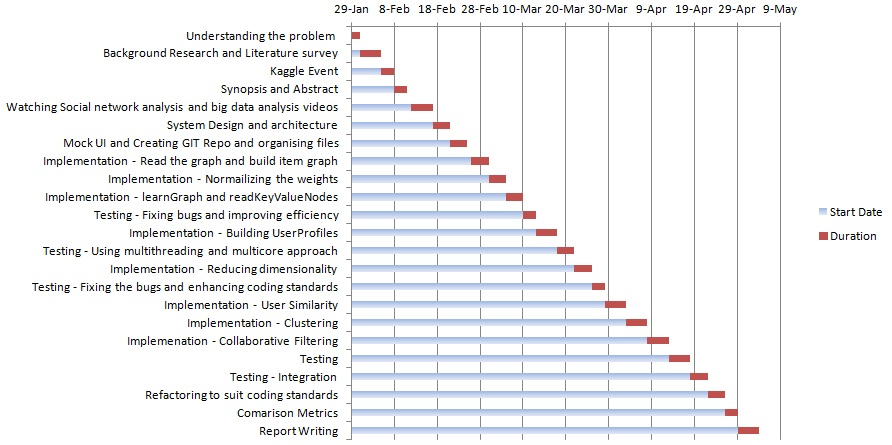
\includegraphics[scale=0.75]{images/gantt.png}
\caption{Gantt chart for the project}
\label{gantt}
\end{figure}

Figure \ref{gantt} presents the Gantt Chart for the timeline of our project.
    \end{projChapter}

\begin{projChapter}{System Design}
\begin{projSection}{Component Diagram}
\begin{figure}[ht!]
\centering
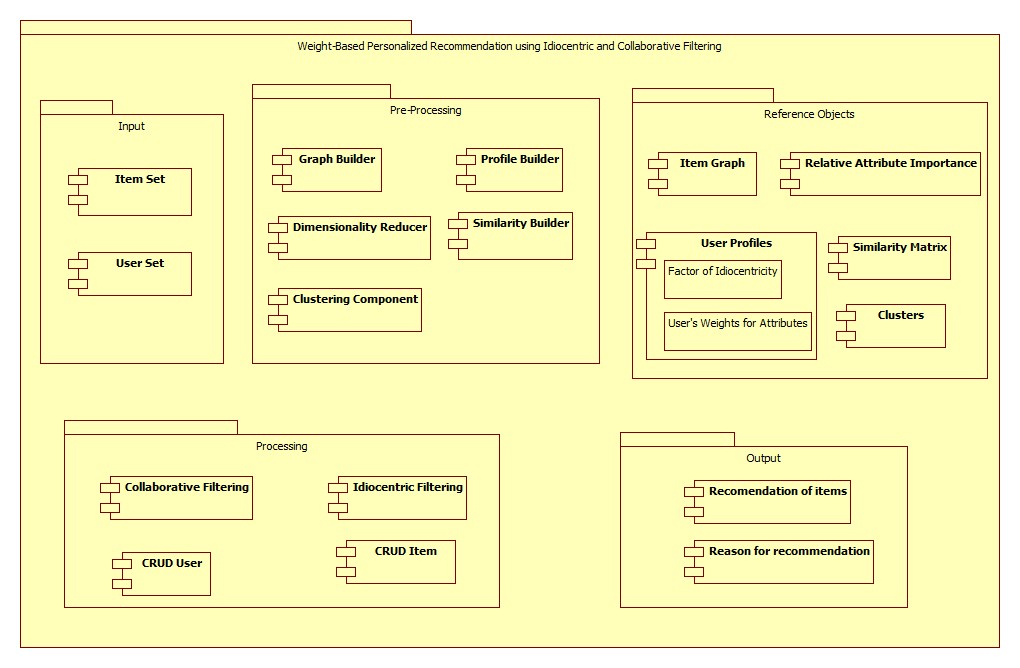
\includegraphics[scale=0.4]{images/component.png}
\caption{Component diagram for the project}
\label{component}
\end{figure}

Figure \ref{component} shows different components or our recommendation system. There are four different components, viz. Input, Pre processing, Processing and Output. The details of each component are as shown in the above figure.
        \end{projSection}
\begin{projSection}{Activity Diagram}
\begin{figure}[ht!]
\centering
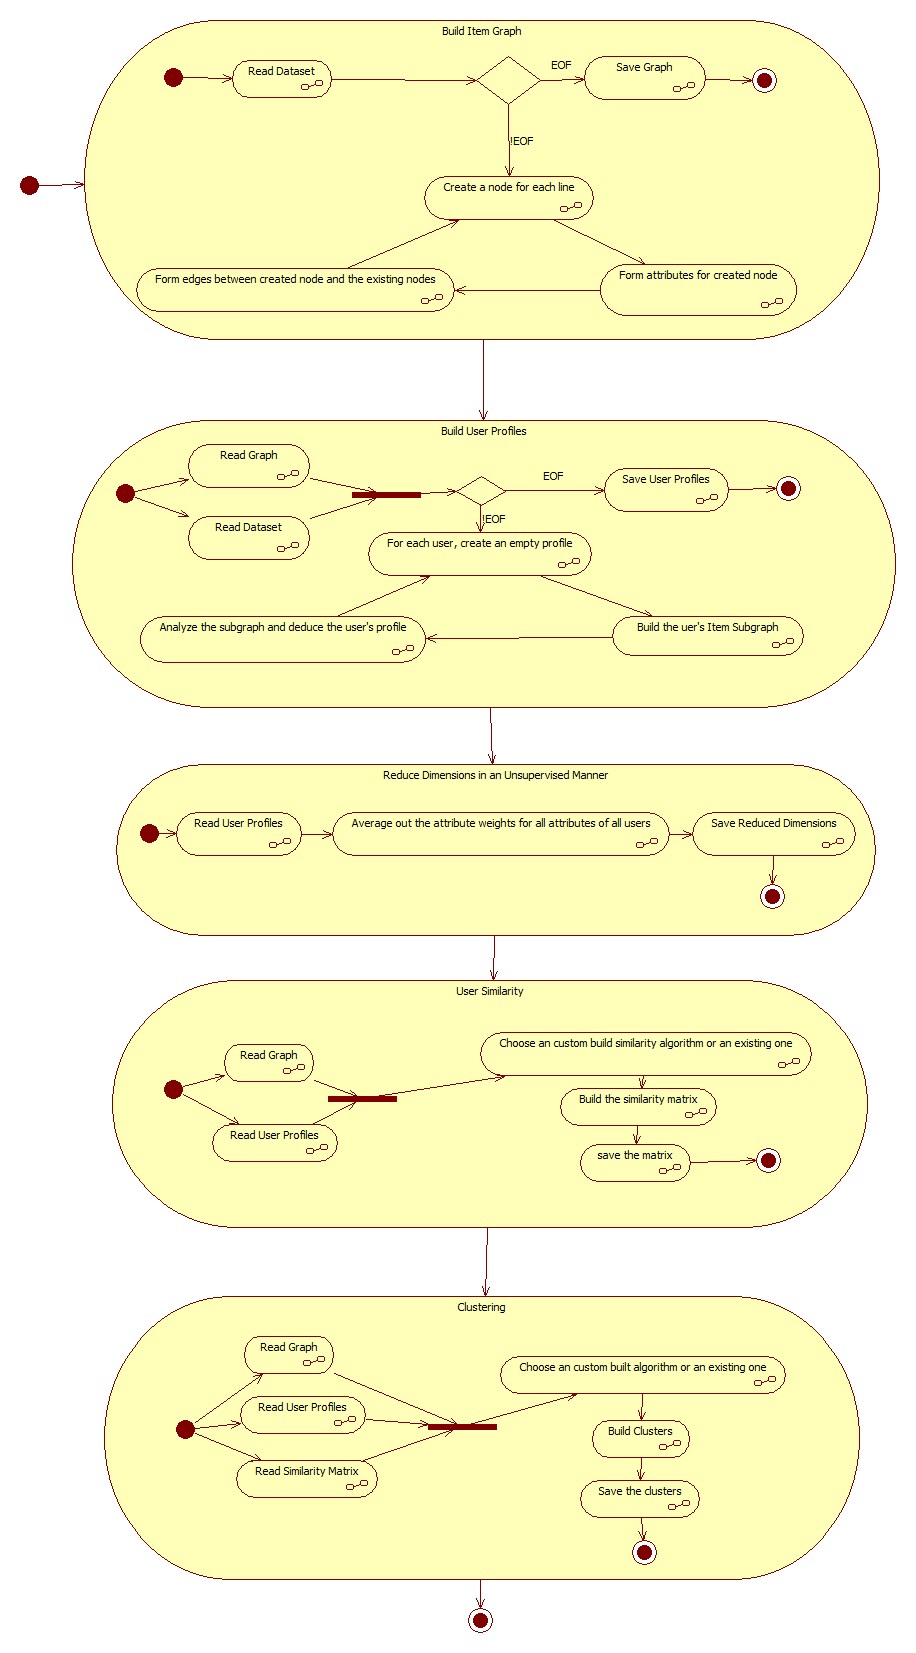
\includegraphics[scale=0.3]{images/activity.png}
\caption{Activity diagram for the project}
\label{activity}
\end{figure}

\end{projSection}

\begin{table}[h]\begin{center}\begin{tabular}{|c|c|c|}\hline
\textbf{Col1} & \textbf{Col2} & \textbf{Col3} \\
\hline
\underline{value 1} & \raisebox{-\totalheight}{\centering

\includegraphics[scale=0.05]{images/pes.png}
\label{pes1}}
 & Sample embedded table:
                    
 \\
\hline
\end{tabular}\end{center}\caption{Sample Table}\end{table}
\end{projChapter}

\begin{projChapter}{Detailed Design}
        The following section describes the design and architecture of the system in detail.
        \begin{projSection}{Building Item Graph}
            As shown in the activity diagram, the flow starts with building the item graph from the item dataset. We build a graph with each node representing an item and each edge representing the common attributes between them. The common attributes that bind the two nodes with its value will be used as an attribute for the edge. Each item is associated with a set of properties.  Each of those properties is mapped on to the graph as the properties of the node. Figure \ref{node} illustrates the concept explained above.
            \begin{figure}[ht!]
\centering
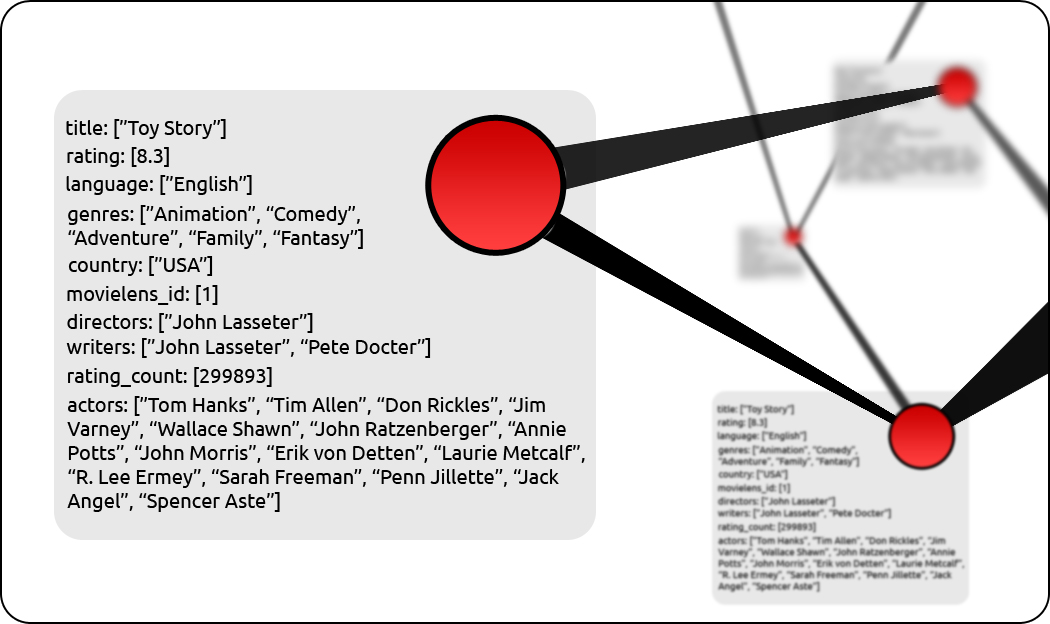
\includegraphics[scale=0.4]{images/node.png}
\caption{The structure of the graph}
\label{node}
\end{figure}

\end{projSection}
\begin{projSection}{Building User Profiles}
            A user is an entity who consumes an item. In this section, we build a profile for each user. The user profile consists of characteristic parameters of the user that quantifies his behavior. In real world, many factors influence the decision of the user to consume a particular item. These factors include the personal choices of the user and recommendation by other users. This scenario is analogous to a customer at a restaurant. The customer might place an order due to recommendations by his friends. His decision is also influenced by what he personally prefers to eat. Generally, the customer does not have equal preferences towards all properties of the food, such as sour, salt, hot and sweet. He has varied levels of liking towards various attributes. Also, the customer might choose to place the order according to his preference or others' recommendation, with a certain probability. We generalize and quantify these behaviors of the customer in order to deduce the characteristic parameters of the customer. 
            ~\\\\
            Each user profile is built by recognizing the relationship among the items that the user has consumed. This relationship is captured in the sub-graph of those items from the item graph. For each user a set of properties are deduced that convey the orientation of the user towards the various attributes of the items. This orientation is quantified in terms of relative attributive importance and relative value importance. This derived knowledge about the user is used to recommend items to that user in both idiocentric and collaborative techniques.
        \end{projSection}
\begin{projSection}{Unsupervised Dimensionality Reduction}
            In this section, we present an empirical approach to perform dimensionality reduction on the dataset. We observe the users' pattern in consuming the items and deduce the importance of an attribute. The importance of an attribute in the item dataset increases as number of users who give higher relative importance to that attribute increases. Hence, the importance of an attribute a in the item set I can be quantified as the mean relative importance of a, taken over all the users u belonging to U. In the previous section, we created a profile for each user. The characteristic parameter w consists of relative weights of attributes for u. The relative importance of an attribute a in the item set I can be computed as follows:
            \begin{figure}[ht!]
\centering
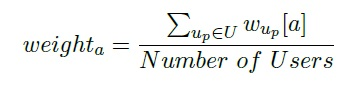
\includegraphics[scale=0.6]{images/attribImportance.png}
\caption{formula for relative attribute importance}
\label{attribImp}
\end{figure}

            ~\\
            A similar argument holds well in case of relative value importance.
            \begin{figure}[ht!]
\centering
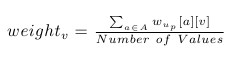
\includegraphics[scale=0.6]{images/valueImportance.png}
\caption{formula for relative value importance}
\label{valueImp}
\end{figure}

\end{projSection}
\begin{projSection}{User Similarity}
            This section explains the collaborative filtering part of the solution. The techniques involved in Collaborative Filtering are based on analyzing a large amount of data on users' activities and predicting what a given user might like. The recommendations can be based on similarity between users or similarity between items. Our algorithm uses similarity between users to perform collaborative filtering. Some of the popular similarity measures are Euclidean Distance, Cosine Similarity, Pearson Correlation and Jaccard Similarity.
            ~\\\\
            Jaccard similarity is a measure used for comparing the similarity of sample sets. Jaccard similarity between two sets A and B is mathematically defined as follows:
            \begin{figure}[ht!]
\centering
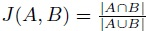
\includegraphics[scale=0.7]{images/jaccard.png}
\caption{formula for jaccard similairty}
\label{jaccard}
\end{figure}

            Each user is associated with a set of items that he has consumed. The similarity between users can be computed just by applying the simple Jaccard similarity between the sets of items for a pair of users. But there is an intrinsic drawback associated with this approach. The approach treats all the items to be equivalent. It is ignorant towards the properties of the items themselves and the relations between them. To include these considerations, we modify the simple formula for Jaccard similarity.
            ~\\\\
            The idea behind the modification is as follows. To compute the similarity between two users up and uq, we compute two induced subgraphs of G. One of them contains the intersecting items of the two users, and the other contains the union of items of the two users. From the two induced subgraphs, we make two aggregated lists of edge attributes, one for each subgraph. Note that the attributes in these lists can repeat. The similarity is calculated as a fraction. To compute the numerator, we iterate through the attributes in the aggregated list for item intersection subgraph. Counting the number of occurrences of these attributes would implicitly mean that we are considering all the attribute as equals. But, the users give varied levels of importance to the attributes. Hence, for each attribute in the aggregated list, we sum up the corresponding weights from the users up and uq and multiply the sum by the relative frequency of occurrence of the attribute in the aggregated list. We follow a similar procedure to compute the denominator, with the only difference being that we consider the item union subgraph.
            \begin{figure}[ht!]
\centering
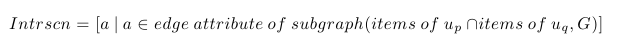
\includegraphics[scale=0.6]{images/intersection.png}
\caption{formula for intersection}
\label{intersection}
\end{figure}

\begin{figure}[ht!]
\centering
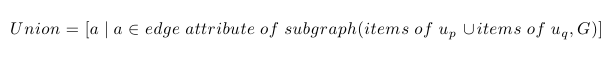
\includegraphics[scale=0.6]{images/union.png}
\caption{formula for union}
\label{union}
\end{figure}

\begin{figure}[ht!]
\centering
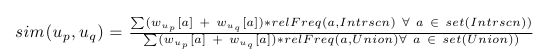
\includegraphics[scale=0.6]{images/similarity.png}
\caption{formula for modified jaccard similairty}
\label{similarity}
\end{figure}

\end{projSection}
\begin{projSection}{Clustering}
            One of the most useful statistical analysis techniques for understanding the user behavior is clustering. This group behavior will help in recommending items that might be of interest to that cluster. The task of grouping users is carried out in such a way that the users belonging to the same group (referred to as a cluster) will have a coherent list of similarity values. These values, in turn, are calculated as explained in the previous section. Here, we use an overlapping clustering approach, where a given user may belong to multiple clusters. Overlapping clustering captures the user interests in vivid attributes.
            ~\\\\
            ~\\
            In the first step, we find out the average similarity between all pairs of users. We then create a trivial cluster for each user and progressively add other users in accordance to the condition that the similarity between a base user and all other users is greater than the average value. On completing this step, we find the clusters exist in duplicates. The duplicates are then removed to obtain the final set of clusters.
        \end{projSection}
\begin{projSection}{Idiocentric Recommendation}
            The idiocentric recommendation algorithm works as follows. We initialize the similarity scores of all the items to zero. Given a user u, we analyze the list of items that u has previously consumed. If a user has consumed an item i, it is very likely that the user might be interested to consume the neighbors of i, but not to equal extents. The extent to which the user might be interested to consume a neighbor not only depends upon the similarity between the items, but also upon the weight that the user gives to the common features between the items. The common features between the items are captured as the property of the edge between them. Hence, we increment the score of each neighbor by the weight that the user gives to each property of the edge. After updating all the nodes, we create an associative array of items and their score. Note that the associative array does not contain the items that are already consumed by the user. We then normalize the scores by dividing all the scores by the maximum score.
        \end{projSection}
\begin{projSection}{Collaborative Filtering}
            Collaborative Filtering (CF) is a collection of techniques that are used in recommending items to users based on the ratings of other users. CF techniques are by far the most successful techniques in recommending items to users. The core idea behind CF techniques is the concept of similarity. The recommender systems generally use two forms of similarities: user-based similarities and item-based similarities. These techniques generally use a standard metric, such as Euclidean Distance, Cosine Similarity, Pearson Correlation or Jaccard Similarity. Once a similarity matrix is built, these systems use various algorithms to generate recommendations. In this project, we have used an extended version of Jaccard similarity. The algorithm that we have developed uses user-based similarity. Our algorithm begins by iterating through all the clusters. A cluster houses many users. Each user is associated with a list of items that he has consumed. For each user up in each cluster c, we increment the score of each item i consumed by up, by the similarity between u and up. Note that the clusters we obtained are overlapping. That is, a single user can belong to multiple clusters. If the given user u1 is very similar to another user u2, then u2 will appear in majority of the clusters where u1 is present. This implies that the score for the items consumed by u2 is naturally boosted, since u2 is presented in most of u1's clusters and the similarity between u1 and u2 is high.
        \end{projSection}
\begin{projSection}{A weighted combination for recommendation}
            The previous sections dealt with generating egocentric and collaborative recommendations for the user. Both the algorithms predict a rating for each item that a user has not consumed. Hybrid Recommendation involves combining the idiocentric and the collaborative scores list of hybrid scores, by means of weighted combination of corresponding items from both the lists. Since we are merging the lists that signify idiocentric behavior and group behavior, we choose alpha as the weight. In one of the previous sections, we had defined alpha as the probability with which the user up decides upon an item purely based on his preferences. alpha quantifies how idiocentric a user is. Hence, assign a weight alpha to idiocentric ratings and (1 - alpha) to collaborative ratings.
            ~\\\\
            We propose two methods by which the lists can be combined:
            
\begin{itemize}
  \item Rank based weighted average:
                    ~\\
                    In this approach, we take a weighted average of ranks of each item and sort the items in the decreasing order of their composite ranks. As mentioned earlier, we assign a weight alpha to idiocentric rating and (1 - alpha) to collaborative rating. The following formula mathematically describes the operation:
                    \begin{figure}[ht!]
\centering
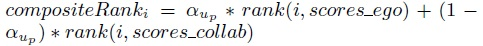
\includegraphics[scale=0.8]{images/compositeRank.png}
\caption{composite rank-based}
\label{compositeRank}
\end{figure}


  \item Score based weighted average:
                    ~\\
                    In this approach, we take a weighted average of ratings of each item and sort the items in the decreasing order of their composite ratings. As mentioned earlier, we assign a weight alpha to idiocentric ratings and (1 - alpha) to collaborative ratings. The following formula mathematically describes the operation:
                    \begin{figure}[ht!]
\centering
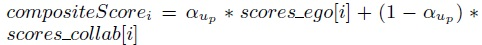
\includegraphics[scale=0.8]{images/compositeScore.png}
\caption{composite score-based}
\label{compositeScore}
\end{figure}


\end{itemize}

            Rank based weighted average method can be used to provide recommendations to the user in the order of their ranks. But predicting the rating that the user might give to an item tends to be relatively hard. Consequently, evaluating the accuracy of our algorithm also tends to be relatively hard. Hence, in our experiments, we use the score based weighted average method to predict the rating that a user might give to a previously unseen item.
        \end{projSection}
\end{projChapter}

\begin{projChapter}{Hurdles: Design Decisions and Optimization}
\begin{projSection}{Git Versioning System}
            In software development, Git is a distributed revision control and source code management (SCM) system with an emphasis on speed.  In our earlier projects, we had used Git in a minimalistic manner, where we used only local repositories to maintain our code. In this project we had to learn more about handling remote repositories on github. We encountered many problems in branching and merging of the code as we had to simultaneously handle many datasets. Our code, commits and branches can be found at 
            ~\\
            https://github.com/vijeshm/recommendation-algorithm-fyp.
        \end{projSection}
\begin{projSection}{MockUp UI}
            We had two tool choices, MockUp and Pencil for creating the UI mockup on Ubuntu. We initially built the UI mockup using Mockup tool but it wasn't sufficiently powerful for our requirements. Hence we modified the mockup using Pencil tool.
        \end{projSection}
\begin{projSection}{Choosing Language}
            In order to quickly and easily implement our algorithm, we had to choose a language designed for code readability, simplicity and robustness. Hence we had three choices, Python, Jython, Cython and R. Finally we decided to use Python as our implementation language for the reasons and tradeoffs mentioned below:
            
\begin{itemize}
  \item \underline{Python v/s R:} The R is widely used among statisticians and data-miners for data analysis. In contrast to Python, R has less support in terms of extensibility, libraries and communities. More insights about other tradeoffs can be found at  pandas.python.org.
  \item \underline{Python v/s Jython:} We had initially thought of using a database to store the reference structures that we generated. Jython was primarily considered as an option as it could be linked with the databases easily. Since Jython uses compiled codes, it was expected to be relatively faster.  But we chose against going with databases, as discussed in next section.
  \item \underline{Python v/s Cython:} Using Cython would have made the execution faster, but it takes lot of time to code and optimize it. Due to project timeline, we could not implement it. Later we found out that integrating the Cython code with the UI code was a huge task by itself.
\end{itemize}

\end{projSection}
\begin{projSection}{Databases}
            We had initially thought of using a graph database to store the dataset and the reference structures. Referring to http://en.wikipedia.org/wiki/Graph\\\_database, HyperGraph and ArangoDb were the most suited ones to our application. But we decided to against the databases, since the read and write time for a database is far greater than that of an in-memory object. The available machines today are capable of managing huge in-memory objects.
        \end{projSection}
\begin{projSection}{Genericity}
            Generally, the development that takes place for these kind of problems are dataset specific. During the development, we identified the parts which can be generalized and abstracted them to work for any generic dataset. In order to bring this about, we put certain constraints on the input dataset formats, such as mandatory "id" field for each item in the dataset. The details of more such constraints can be found in Input requirements section.
        \end{projSection}
\begin{projSection}{32-bit Addressable Woes}
            During the initial stages of development, we had used a 32-bit addressable OS to execute our code. Apparently the size of our graph object exceeded 4GB and there was a Memory Error exception. This motivated us to optimize the algorithm and data-structures. In the course of 3 days, we realized that we were using a 32-bit addressable OS. We solved the problem by porting our code to a 64-bit OS.
        \end{projSection}
\begin{projSection}{Graph}
\begin{projSubSection}{Writing huge memory objects as a pickle file}
                The pickle module takes a lot of memory to stringify objects. We tried to stringify the huge graph objects on an 8GB RAM machine but the memory was still insufficient and the graph object by itself took a lot of space. The solution to the problem was to write only the required information about the graph manually onto a file.
            \end{projSubSection}
\begin{projSubSection}{Graph Formats}
                A graph object can be stored on a disk in many formats such as:
                
\begin{itemize}
  \item GEXF
  \item GDF
  \item GML
  \item GraphML
  \item Pajek NET
  \item GraphViz DOT
  \item CSV
\end{itemize}

                We tried to export the graph objects onto these formats, but we encountered the same problems as we did in the pickle export.
            \end{projSubSection}
\begin{projSubSection}{Graph Storage}
                Due to the problems mentioned above, we decided to export the graph as an edgelist along with its properties. Each line in the file is of the form:
                ~\\
                node1 node2 properties
                ~\\
                This file consumed 1.5 GB of space on the disk. On enumeration of the attributes and values of the edge properties, we were able to reduce the file size to 982 MB. But this still proved to be very large on converting it back to an in memory object. To overcome these problems, we had to come up with the new and innovative solution. We exploited the graph structure and used the technique of reverse indexing to get the size down to 2.0 MB. The reverse indexed structure is as follows.
                ~\\
                *insert keyValueNode structure here*
            \end{projSubSection}
\end{projSection}
\begin{projSection}{Categorization of non-categorical Data}
            Attributes that are of integers, floating point and time data types fall under numerical or non-categorical data. But our algorithm is designed to work for categorical data. Hence there is a need to convert this data into categories. We referred "Data Clustering Theory, Algorithms and Applications by Guojun Gan, Chaoqun Ma, Jianhoug Wu" in order to achieve this. The method that they propose uses K-Means clustering to categorize the numerical data iteratively. This proved to be a time costly operation. Hence we came up with time efficient clustering solution that serves our needs.
        \end{projSection}
\begin{projSection}{Parallelization of Algorithms}
            The algorithm was designed keeping in mind the possibility of parallelization. Many parts of the approach were inherently parallelizable. We came up with 3 solutions for parallelization of building user profiles, as listed below:
            ~\\\\
            For each user, a new process is spawned for building the corresponding user profile. This induced a highly coarse granularity between the processes. In turn, there was a drastic increase in the CPU usage, RAM and Swap space. Figure \ref{sysmon} illustrates the point.
            \begin{figure}[ht!]
\centering
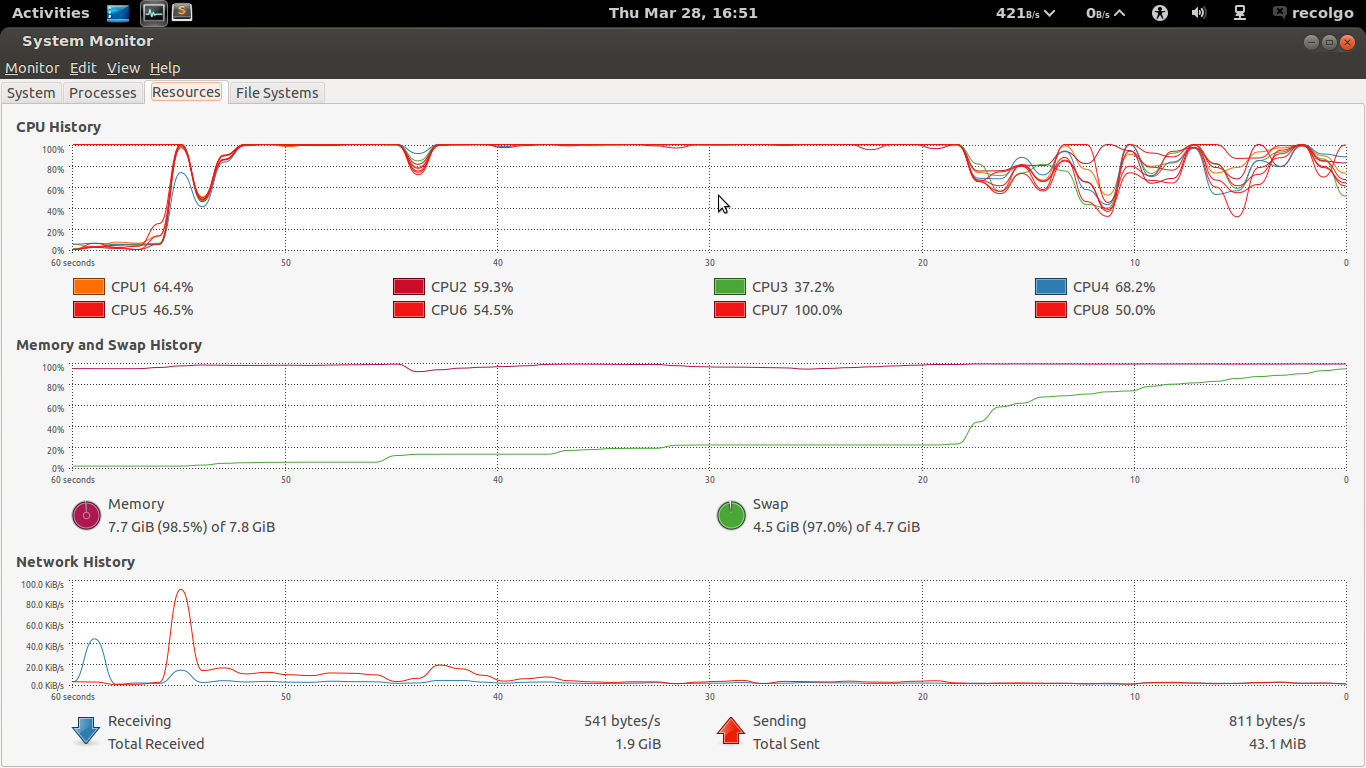
\includegraphics[scale=0.35]{images/sysmon.png}
\caption{state of the system during execution}
\label{sysmon}
\end{figure}

            We then used a limited pool of 4 processes (using the Pool module from multiprocessing), and assigned jobs to these 4 processes. This method couldn't be used to recursively parallelize the algorithm. The problem with this technique was sharing the data. When we passed a reference to a data structure, the data present in the object could be read. But when we write the data back, the action was not being reflected in the parent process. Hence, this approach wasn't suitable either. The memory consumed decreased and the CPU usage was reduced considerably (approximately 2GB and 40\\\% usage on 4 cores).
            ~\\\\~\\
            Execution time for building basic user profiles: 
            ~\\
            Linear execution: 11s
            ~\\
            multithreaded: 44s
            ~\\
            i.e. a factor of 0.25
            ~\\\\
            Another solution was to create multiple threads. This would allow us to share data easily, and doesn't create much overhead in terms of inter-process communication. The procedures can be recursively parallelized. But this method also introduced a coarse granularity. 
            ~\\\\
            Considering all the above mentioned factors, we decided to go with the linear execution of the algorithm, though it can be parallelized.
        \end{projSection}
\end{projChapter}

\begin{projChapter}{Implementation}
        The following section describes the implementation details of the design we have come up with.
        \begin{projSection}{Item Graph}
            In our initial phase, we had built a graph object of all the items as nodes with the common attributes between them as connecting edges. But this method proved costly in terms of space. The whole graph object used to get stored in memory and hence to make it more memory efficient we thought of changing the way of data representation.
            ~\\\\
            The data structure we came up with to represent the item dataset was of key-value-node pair. By reverse indexing the data set, we observed that the amount of space it occupied was lesser. The key here mean the attribute and the value is the value of the attribute. Node describes the items that are associated with that particular attribute-value pair.
            ~\\\\
            For example, say we have item1 and item2 having common attributes a2 with value v1 and similarly item3 and item4 with a2 and v3 respectively. In our key-value-node pair, this can be represented as:
            *insert keyValueNodes structure here*
            ~\\\\
            The item dataset consists of both categorical and non-categorical data. The categorical data will be either string or boolean type (Eg: Director and Like, respectively). Non-categorical data includes all the numerical attributes. (Eg: rating, year, timestamp).  The following algorithms explain the approach for the two types of data:
            
\begin{itemize}
  \item For categorical data:
                    \begin{figure}[ht!]
\centering
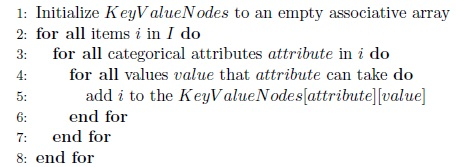
\includegraphics[scale=0.8]{images/categorical.png}
\caption{building keyValueNode structure for categorical data}
\label{categorical}
\end{figure}


  \item For non-categoricla data:
                    \begin{figure}[ht!]
\centering
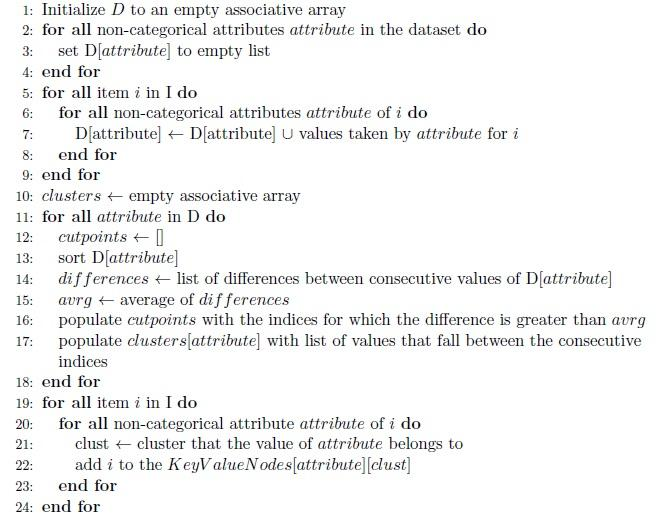
\includegraphics[scale=0.6]{images/noncategorical.png}
\caption{building keyValueNode structure for categorical data}
\label{noncategorical}
\end{figure}


\end{itemize}

\end{projSection}
\begin{projSection}{User Profile}
            Building user profiles from the user dataset is a major task as it eventually helps in idiocentric recommendation. User profiles are built by the data obtained from the user dataset. It takes into account the orientation of the user towards the value of a particular attribute as well as the attribute itself. The relative attributive importance and the relative value importance together define the attitude of the user towards the attributes in the item dataset. The personalized user profiles will be built using the key-value-node reference structure generated on building the item graph. The algorithm starts with initializing an empty associative array for each user. The relative attributive importance of each attribute is computed eventually for all the users. In computing the profiles for each user, we consider the ratings of items in the intersection between the user's consumption list and the list of key-value-nodes in the way illustrated by the following algorithm.
            \begin{figure}[ht!]
\centering
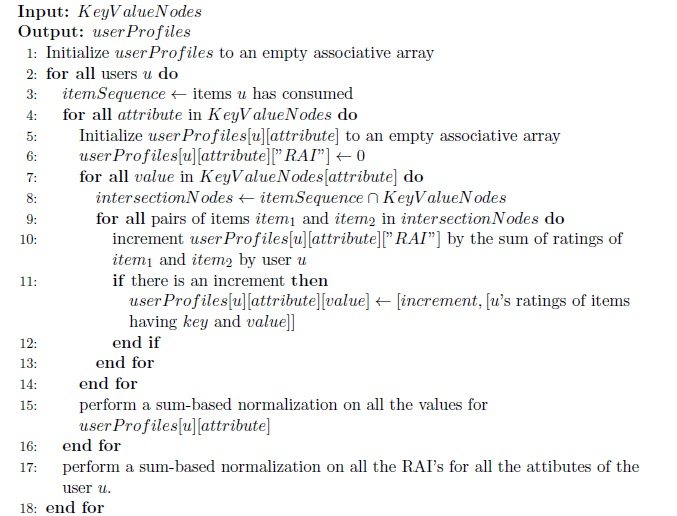
\includegraphics[scale=0.8]{images/userProfile.png}
\caption{Algorithm to build userProfile}
\label{userProfile}
\end{figure}

\end{projSection}
\begin{projSection}{Reduce Dimensionality}
            The reduction in the dimensionality of the dataset is performed for both attributes and values. Attribute dimensionality reduction is the relative importance of an attribute taken over all the users. In other terms it defines the mean relative importance of an attribute taken over all the users. In the same manner, value dimensionality reduction is also computed, which quantifies the mean relative importance of a value of an attribute taken over all the users. The following algorithms describe the two concepts in a programmatic manner.
            \begin{figure}[ht!]
\centering
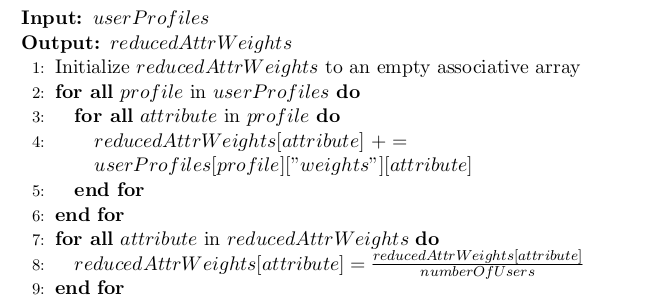
\includegraphics[scale=0.6]{images/dimredattrib.png}
\caption{Algorithm to reduce dimensionality of attributes}
\label{dimredattrib}
\end{figure}

\begin{figure}[ht!]
\centering
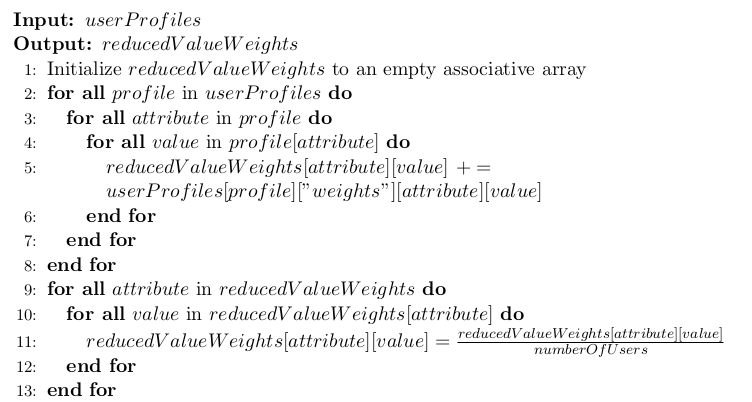
\includegraphics[scale=0.6]{images/dimredvalue.png}
\caption{Algorithm to reduce dimensionality of values}
\label{dimredvalue}
\end{figure}

\end{projSection}
\begin{projSection}{User Similarity}
            To compute the similarity between two users up and uq, we compute two induced sub-graphs of G. One of them contains the intersecting items of the two users, and the other contains the union of items of the two users. From the two induced sub-graphs, we make two aggregated lists of edge attributes, one for each sub-graph. Note that the attributes in these lists can repeat. The similarity is calculated as a fraction. To compute the numerator, we iterate through the attributes in the aggregated list for item intersection sub-graph. Counting the number of occurrences of these attributes would implicitly mean that we are considering all the attribute as equals. But, the users give varied levels of importance to the attributes. Hence, for each attribute in the aggregated list, we sum up the corresponding weights from the users up and uq and multiply the sum by the relative frequency of occurrence of the attribute in the aggregated list. We follow a similar procedure to compute the denominator, with the only difference being that we consider the item union sub-graph. The algorithm below shows how it is implemented:
            \begin{figure}[ht!]
\centering
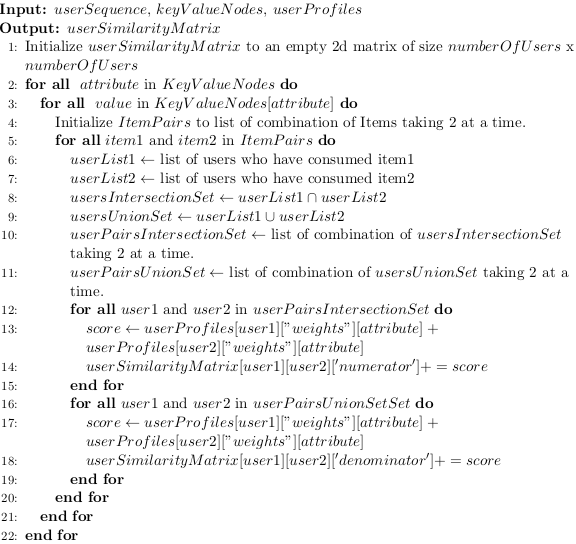
\includegraphics[scale=0.6]{images/userSimilarity.png}
\caption{Algorithm to compute user similarity}
\label{userSimilarity}
\end{figure}

\end{projSection}
\begin{projSection}{Idiocentric Recommendation}
            In this section, we predict the ratings that a user would give to an item considering idiocentric behavior. userWeights is an associative array that contains the weights given by that user for different attributes as well as values taken by that attribute. itemList is the list of items for which rating has to be predicted. The algorithm computes the scoreIdio for each item in the itemList using the userWeights associated with the attribute and their corresponding values of the item.  Finally, to predict the rating of a given item, we take the dot product of score and ratings and divide it by sum of ratings in order to normalize. The algorithm is as follows:
            \begin{figure}[ht!]
\centering
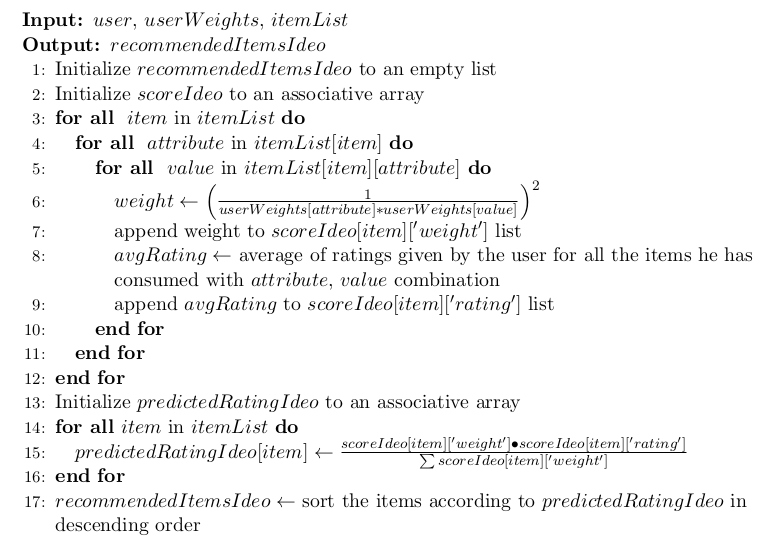
\includegraphics[scale=0.6]{images/idiocentric.png}
\caption{Algorithm to produce idiocentric recommendation}
\label{idiocentric}
\end{figure}

\end{projSection}
\begin{projSection}{Clustering}
            In the clustering algorithm, we cluster the users based on interest towards a particular attribute. Each user may belong to more than one cluster. i.e, we are performing an overlapping clustering technique. The method is as follows. The first step involves calculating averageSimilarity between all the users in order to set the threshold. This is done by averaging all the values in the userSimlarityMatrix computed in previous step. In the second step, a pair of users is combined to form one cluster if their similarity value is greater or equal to threshold. The algorithm is as follows:
            \begin{figure}[ht!]
\centering
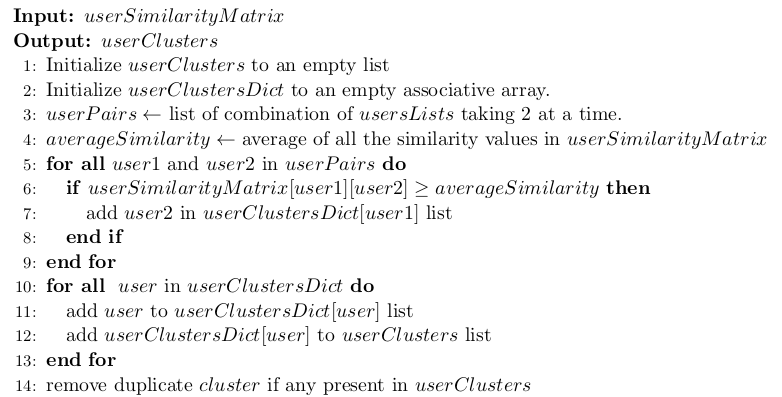
\includegraphics[scale=0.6]{images/clustering.png}
\caption{Algorithm to cluster the users}
\label{clustering}
\end{figure}

\end{projSection}
\begin{projSection}{Collaborative Filtering}
            Collaborative filtering determines the rating a user might give to an item, considering the ratings given by other users who are similar to user under consideration. The algorithm takes userSimilarityMatrix, clusters, itemList as input. itemList is the list of items for which rating has to be predicted. For each item, collaborative filtering algorithm builds a vector of ratings (given by other users) and a vector of similarity values between the given user and other users. Finally, collaborative rating is predicted by taking a dot product of these vectors and normalizing by sum. The algorithm is as follows:
            \begin{figure}[ht!]
\centering
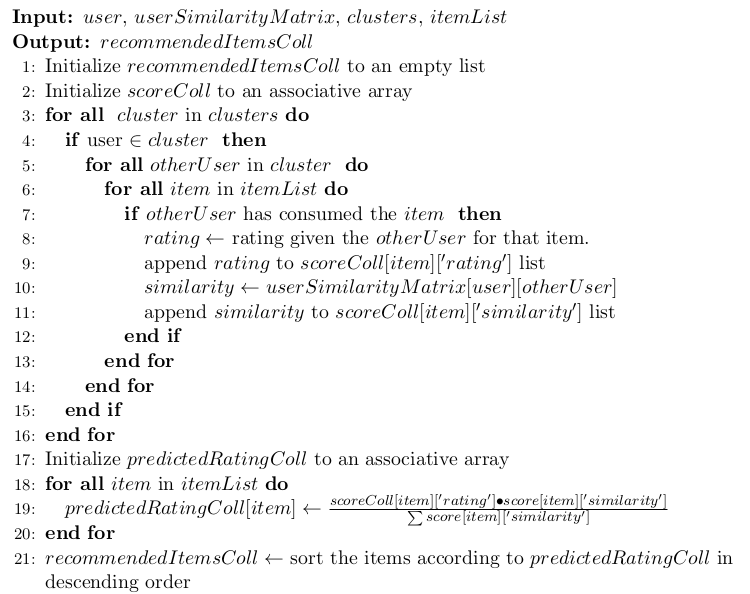
\includegraphics[scale=0.5]{images/collaborative.png}
\caption{collaborative filtering algorithm}
\label{collaborative}
\end{figure}

\end{projSection}
\end{projChapter}

\begin{projChapter}{and so on...}
        so forth...
    \end{projChapter}



\end{document}
